\section{Unity3D project}
The project has been built using Unity3D version 5.2.
While newer versions might be able to run the simulation, we can guarantee that it does run on this version.\\

\subsection*{Download and Import}
The project can be found on github following this url: \url{https://github.com/inau/autonomous/tree/master/Intersection/IntersectionManagement2D}.\\
This is a subdirectory so cloning should be done from the parent directory.\\
When importing into the game engine use the folder 'IntersectionManagement2D'.\\

\subsection*{Project Structure}
\noindent
Unity projects contain a 'ProjectSettings' folder and an 'Assets' folder. The assets contain all the interesting stuff.\\
\noindent
Our simulation has been structured into 'Core' package and 'Control' package.\\
\subsubsection*{Core}
This package has two folders, one which contains the essentials for modelling the intersection and another which contains the essentials for cars.\\
The intersection directory has Origin and destination points, graph representation and an intersection file which combines these components to make up an intersection.\\
The car directory contains interface for car movement and sensors.\\
\subsubsection*{Control}
This folder has controllers for our car model. It contains the reactive controller and older simpler versions.
\pagebreak
\subsection*{Performing Experiments}
To perform similar experiments as we did open up the Unity editor and open up IntersectionManagement2D project.\\
Load the scene named \textbf{'intersection.unity'}.\\
To change test parameters select the Intersection gameobject. This will have the intersection script attached to it, as seen on the following image.\\

\noindent
The check boxes in the top are the ones that determine the experiment type, especially 'Traffic Light Mode' and 'can turn'. The feature 'write results' creates files with the experiment results in the project directory.
The values below are both variables and real-time values from the simulation.\\

\begin{center}
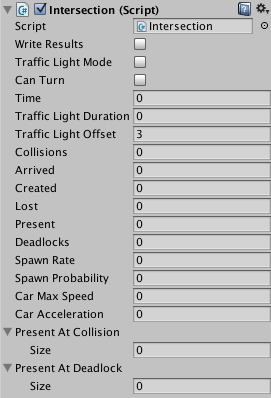
\includegraphics[scale=.5]{img/intersection-panel}
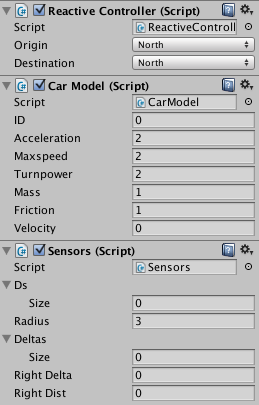
\includegraphics[scale=.5]{img/car-prefab}\\
\textit{\textbf{Intersection script to the left, Car prefab to the right}}
\end{center}

\noindent
To change additional test parameters change values on the car prefab found in the resources folder. The prefab is a way to define template objects that are reused.\\

\noindent
Both sensor and car model can be tweaked. Remember that 1 distance unit in unity translates to 5.5 meters in the real world.
